\subsection{Goals and Objectives}
%The objective is ``\textbf{Automated Risk Detection and Mitigation}''

In this proposal, we propose XAI-enabled Vulnerability Detection and
Assessment Framework (XAI-VDA). Instead of resolving complex scenarios
of security vulnerability detection as an binary output of yes and no,
we aim to leverage Explainable AI to amplify the human intelligence in
detecting vulnerabilities and assessing their impacts in software
systems.

In our proposed `Human-in-the-Loop Explainable-AI-Enabled
Vulnerability Detection, Investigation, and Mitigation' (HXAI-VDIM)
system, instead of resolving complex scenario of security
vulnerabilities as an output of an AI/ML model (e.g., a definitive
outcome of yes or no, or a likelihood score for vulnerability degree),
we integrate the security analyst or forensic investigator into the
man-machine loop and leverage the explainable AI (XAI) to combine AI
and Intelligence Assistant (IA) in amplifying human intelligence in
both proactive and reactive processes. Our philosophy is that {\em "a
  machine and a mind can beat a mind-imitating machine working by
  itself"}~\cite{DBLP:conf/ifip/Brooks77}. Our ultimate goal is that
the proposed HXAI-VDIM system will amplify the human intelligence in
resolving and investigating complex security vulnerabilities. In other
words, HXAI-VDIM integrates both human and machine in an interactive
and iterative loop that utilizes human intelligence to guide the
XAI-enabled system and generate refined outputs -- see Figures
\ref{fig:overview} and \ref{fig:arch}.

Specifically, HXAI-VDIM's workflow is as follows. The Explainable Detection Model is trained via the dataset collected throughout the operations of the system (and in the context of our proposal, IoT system) as well as those from other sources. The trained model is then used to run on the current IoT system. The result of the XAI model will be visualized through a Security Vulnerability Visualization (SVV) model to produce for the human expert the report of observable evidences on the potential vulnerabilities in the IoT system under study.  
Unlike traditional ML model, the Explainable Detection model used for vulnerability detection, investigation, and mitigation (VDIM) {\em produces not only the detection results but also the connections between the results and the input IoT system indicating the reasons why the model has made that decision}. Specifically, the observable evidences will point to the specific data collected from the potentially vulnerable components (hardware and/or software) in the IoT system that are crucial for the XAI model to come up with the result. For example, in the smart campus IoT system, at the first iteration, the XAI model can point to a long list of different potentially vulnerable components as the root causes. Unlike in the traditional approach where the human expert will sift through the long list with several false negatives, (s)he will be integrated into the VDIM process for the next iteration. The human expert will compare the observable evidences with the potential vulnerabilities identified in the previous iteration to provide the adjustments on those identified vulnerable components. Based on those adjustments, the input to the XAI model in the next iteration will be modified accordingly as well as the parameters of the XAI-enabled Detection Model. The entire process of HXAI-VDIM is repeated until all (detected) vulnerabilities are identified or the human expert is confident about the given system. For security investigation, the forensic expert or security analyst will consult with the observable evidences to produce the final report on the vulnerabilities.


%\begin{wrapfigure}{l}{0.8\textwidth}
\begin{figure}[t]
	\centering
	\includegraphics[width=4in]{hxai-vdim.jpg}
	\caption{Human-in-the-Loop XAI-enabled Vulnerability Detection, Investigation, and Mitigation}
	\label{fig:overview}
\end{figure}
%\end{wrapfigure}
With the Human-in-the-Loop framework, the two key stakeholders (human expert -- forensic investigator and/or security analyst, and automated tool) {\em complement  each other} in producing an effective and efficient VDIM process. {\em The automated tool leverages human intelligence to quickly narrow down the features/factors crucial for the tool. At the same time, human intelligence is amplified with the use of automated tool via XAI and visualization}. To realize our framework, we will pursue the following three key work tasks.

\noindent {\bf Work Task 1. HXAI-VDIM System Design and Implementation} (Section~\ref{section:T1}). In this work task, we will design and develop our HXAI-VDIM architecture to be concretized into a tool-suite of supports on (1) security vulnerability detection that pro-actively scans the potential risks and vulnerabilities; (2) security vulnerability investigation toolset that assists forensic analysts and experts in performing digital (forensic) investigations, tracing, and identifying the attack source of an incident occurrence; and (3) an integrated tool suite for the remedial and mitigation actions in the wake of such security incident.


\noindent {\bf Work Task 2: Proactive Human-in-the-Loop Vulnerability Detection with Explainable AI} (Section~\ref{section:T2}). In this work task, we will design and develop the core components relevant to proactive direction of our HXAI-VDIM architecture. First, we will develop the theoretical framework,
algorithms, and models for proactive vulnerability detection to identify the vulnerable IoT devices in an IoT network. Second, we will investigate and design the XAI model that will provide the vulnerability detection results on the vulnerable IoT devices, and explain why the model predicts such a vulnerability by making connections from the result to the input for such an explanation. Finally, we will develop a Human-in-the-Loop framework that leverages the XAI-based vulnerability detection model to realize our HXAI-VDIM framework shown in Figure~\ref{fig:overview}.  

\noindent {\bf Work Task 3: Human-in-the-Loop, XAI-enabled Digital Forensic Investigation and Mitigation} (Section~\ref{section:T3}) In this work task, we will design and develop the core components relevant to forensic investigation and mitigation (reactive activities). The first module is the software vulnerability scanner. After the vulnerable IoT device is identified and isolated, we start scanning for software vulnerabilities in each isolated device. After software scanning, the forensic expert will use our XAI model to perform forensic investigation and start the mitigation process as needed. Thus, the second module in this work task is the Human-in-the-Loop framework for forensic investigation that is guided by the XAI-enabled Vulnerability Detection Model.

\subsection{NSF Research Objectives and Anticipated Results}

\begin{figure}[t]
    \centering
%    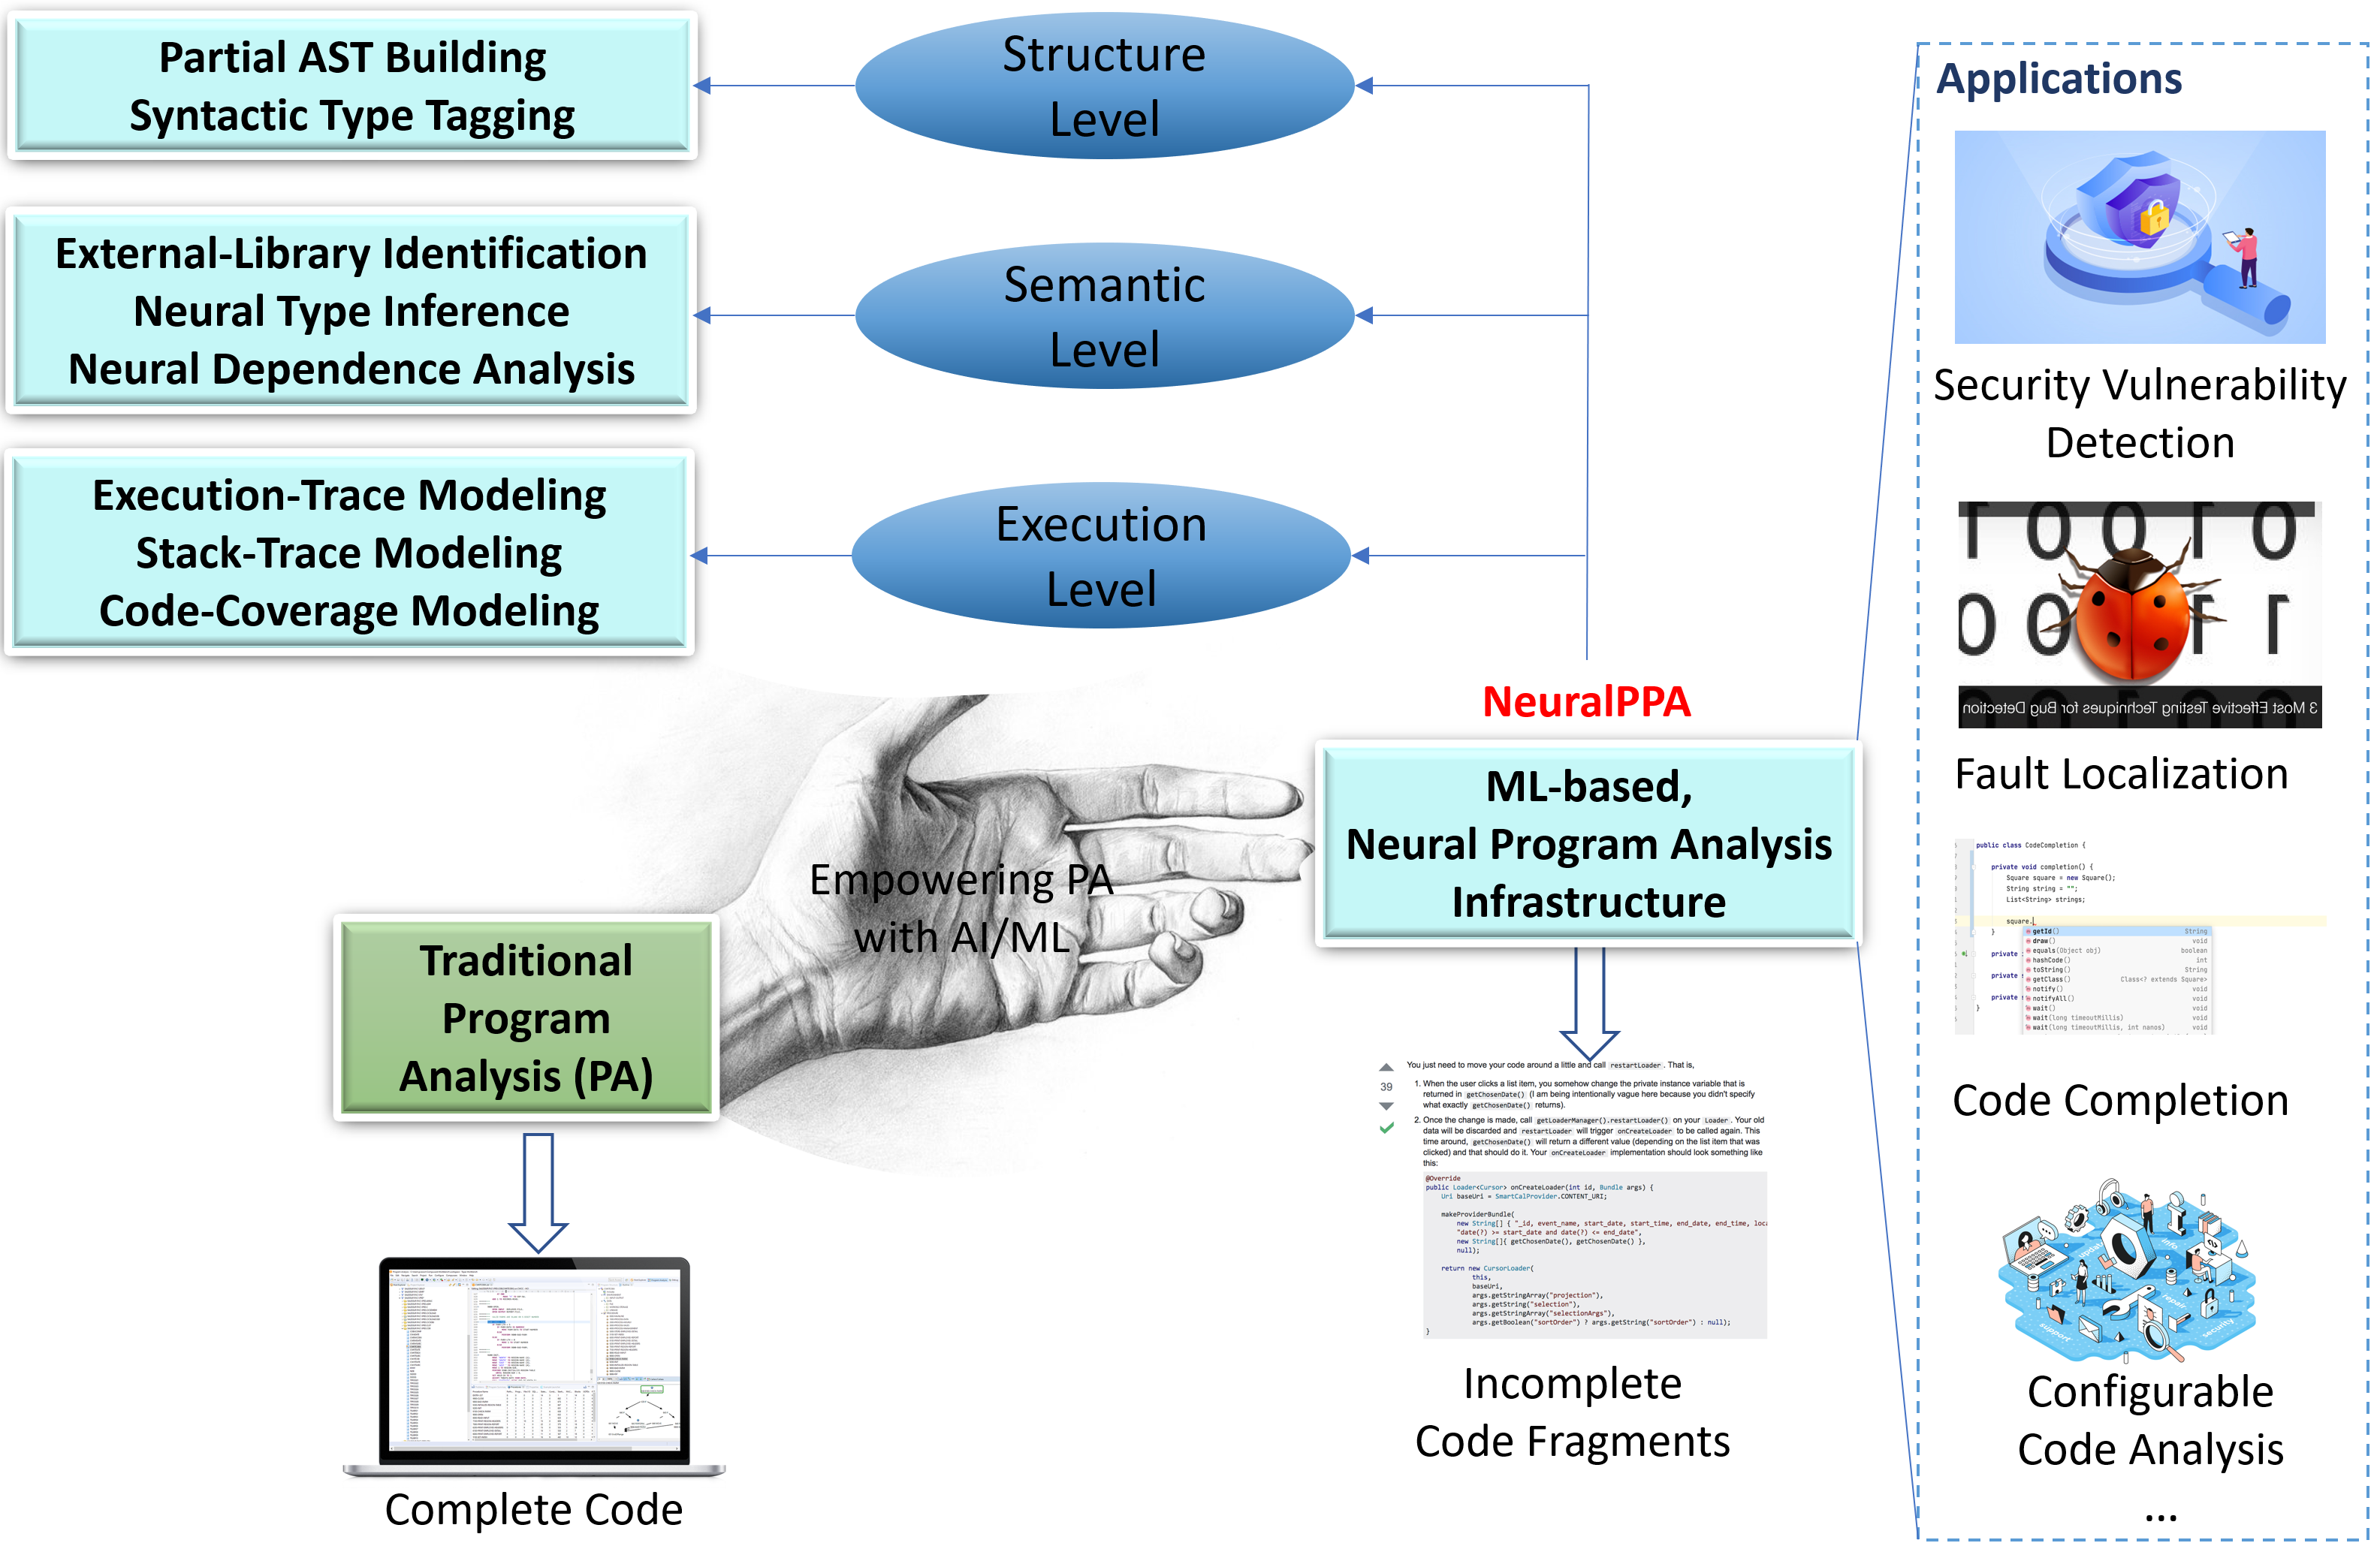
\includegraphics[width=0.83\textwidth]{graphs/neuralppa}
    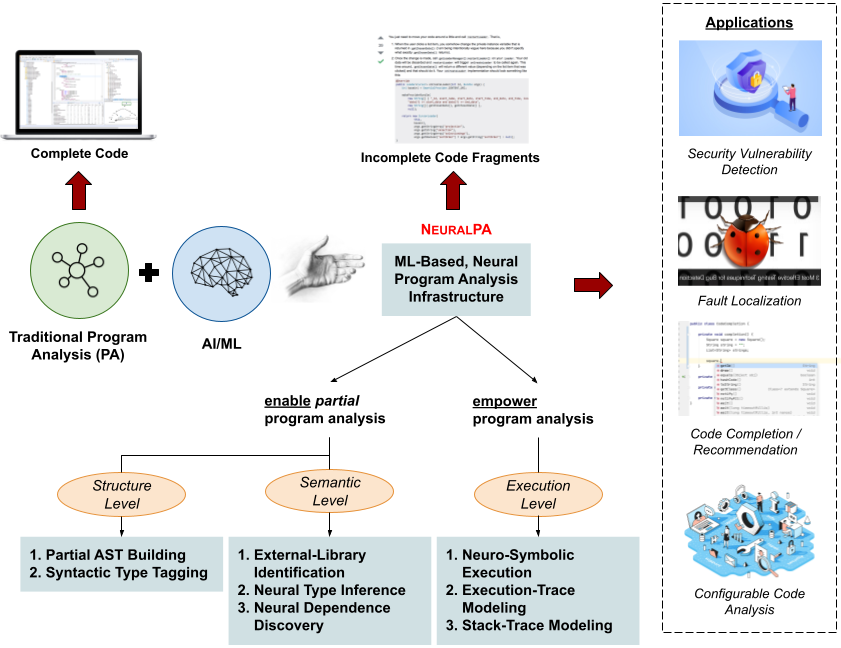
\includegraphics[width=0.92\textwidth]{figures/infra-design-3.png}
%    \vspace{-10pt}
    \caption{{\tool}: Machine Learning-based Program Analysis Infrastructure}
    \label{fig:arch}
\end{figure}


In this proposal, we seek to address these issues and advance the state-of-the-art in traditional program analysis by means of {\tool}, a {\em \underline{Neural} Network-Based \underline{P}rogram \underline{A}nalysis} infrastructure. We aim to establish {\em a scientific foundation, novel methodologies, frameworks, models, and algorithmic solutions for neural program analysis}. Our primary focus areas can be summarized as follows: 

%(1) {\bf Enabling analysis of incomplete code fragments}, i.e., partial program analysis;
(1) {\bf enabling analysis of incomplete code fragments}, i.e., partial program analysis;

%(2) {\bf Empowering existing PA tools by making them more sound and complete}. 
(2) {\bf empowering existing PA tools with advanced AI/ML
%techniques
} to make them more sound and complete.

\noindent Figure~\ref{fig:arch} illustrates the 
%general 
framework for {\tool}, which will allow the construction of efficient program analysis techniques for (partial) code, also based on which downstream 
%software engineering 
SE applications can be built.


\begin{center}
    \begin{minipage}{36em}
The key philosophy that drives our work is that the {\em structural, semantic, and symbolic execution-level analyses of partial code can be learned from the analysis of entire programs in the wealth of information obtained from ultra-large-scale, open-source software repositories}.
    \end{minipage}
\end{center}



We draw motivation for such a data-driven, learning-based approach from the following. First, ultra-large-scale software repositories, e.g., GitHub (7M+ projects) and SourceForge (700k+ projects), contain an enormous collection of programs. These repositories amount to 1B+ lines of code, 10M+ revision logs, and 3M+ issue reports. This wealth of knowledge is an excellent source for {\tool}. Hindle {\em et al.}~\cite{naturalness-icse12} have shown that code has high repetitiveness and predictability and can be captured well by statistical models. Thus, we expect to build ML/DL models to learn from those repositories. 
Second, the PI group reported a high repetitiveness level for AST code structure in open-source projects~\cite{icse15}. Thus, {\tool} infrastructure could help learn structure-level information from the ASTs extracted for whole programs in the existing code repositories and infer data types, partial ASTs for partial programs. Third, in an empirical study on the repetitiveness, containment, and composability of PDGs in open-source projects, the PI group~\cite{msr16} reported that among 17.5M PDGs with 1.6B PDG subgraphs, 14.3\% of the PDGs have all of their subgraphs repeated across different projects. Furthermore, in 15.6\% of the PDGs, at least 90\% of their subgraphs are likely to have appeared before in other projects. 
%Thus, {\tool} could learn from PDGs with complete program dependencies retrieved from existing code repositories and derive the dependencies for the (partial) code fragment under study. The PI group also reported a high repetitiveness level for AST code structure in open-source projects~\cite{icse15}.
Thus, {\tool} could learn semantic-level information from the PDGs with complete program dependencies retrieved from existing code repositories and infer such dependencies for the partial code fragment. Execution can also be modeled
from the ones in the past.

%\textcolor{red}{Add a line for execution-level}.

%Finally, such a program analysis infrastructure like {\tool} can be
%drawn from the spirit and successes of the approaches in natural
%language processing (NLP). For example, at the lexical level, the task
%of deriving the token types for source code tokens could be analogous
%to the part-of-speech (PoS) tagging in NLP. At the syntax level, the
%task of learning the syntactic structure in AST of the partial code
%can be inspired by the approaches to build parse trees for
%natural-language texts. At the semantic level, the partial program
%dependence analysis infrastructure is similar in spirit to the neural
%network-based dependency parsing in NLP, which learns the dependencies
%signifying the semantic relationships between words in a sentence from
%text corpora. In addition, there is much room for innovations in AI/ML
%for source code.

Broadly, the proposed program analysis infrastructure, \tool, draws inspiration from the successes of the neural network-based approaches in the field of natural language processing (NLP). For example, the task of deriving the data types for the source code tokens is analogous to the part-of-speech (POS) tagging task in NLP. At the syntactic level, learning the syntactic structure, i.e., the ASTs for partial code can be inspired by the approaches to infer parse trees for natural language texts. At the semantic level, the partial program dependence analysis infrastructure is similar in spirit to neural network-based dependency parsing in NLP, which learns the dependencies signifying the semantic relationships between words in a sentence from text corpora. In addition, there is much room for innovations in AI/ML for source code.


To accomplish these tasks, we propose the following thrusts of research in {\tool} (see Table~\ref{tab:milestones}):

\vspace{3pt}
%\noindent \textbf{Thrust 1. Neural Structural Analysis Infrastructure
%  \code{NeuralStruct}.} ({\em Section~\ref{}}) Source code has
%well-defined structures and semantics. Thus, the basic infrastructure
%in {\tool} is the neural structural analysis component.  This
%component has two main tasks. First, it learns from the syntactic
%structures of the complete code in the training dataset collected from
%large-scale code repositories, to derive the abstract syntax tree
%(AST) that best represents the syntactic structure of the given
%partial code, i.e., with the highest likelihood/probability.  The
%traditional lexical analyzer still works for partial code due to the
%independence nature of lexical tokens. The second task of this
%component is to tag the code tokens with the types of the syntactic
%units including the statement types (\code{if}, \code{for}, etc.),
%variables, fields, methods, classes, etc. Both of the tasks can be
%performed with our learning-based approaches in a dual-learning
%manner.

\noindent \textbf{Thrust 1. Neural Structural Analysis Infrastructure.} ({\em Section~\ref{sec:thrust1}}) Source code has a well-defined structure and semantics. Thus, the basic infrastructure in {\tool} is the neural structural analysis component, which primarily has two tasks. First, it learns from the syntactic structures of the complete code in the training dataset collected from large-scale code repositories, to derive the abstract syntax tree (AST) that best represents the syntactic structure of the given partial code, i.e., with the highest likelihood/probability. The traditional lexical analyzer still works for partial code due to the independence nature of lexical tokens. The second task of this component is to tag the code tokens with the types of the syntactic units including the statement types (\code{if}, \code{for}, etc.), variables, fields, methods, classes, etc. Both of the tasks can be performed with our learning-based approaches in a dual-learning manner.
  
\vspace{3pt}
\noindent \textbf{Thrust 2. Neural Semantic Analysis Infrastructure.}
({\em Section~\ref{sec:thrust2}}) The basis components for several
analysis techniques on the semantics of the program include the
following:

1) the identification of the APIs of the external libraries in the
external references in the partial code: this is needed because the
partial code contains the undeclared reference and/or
declaration/reference ambiguity without explicit declaration of the
APIs in the external libraries.

2) the inference of the type information for the entities in the
partial code: due to the ambiguity in the declaration, the types of
the variables and statements are not always obviously
identified. Thus, the type inference is a basic service within
{\tool}.

3) the inference of the program dependencies among the statements in
the partial code: several program analysis techniques are based on the
program dependencies, which are not always obtainable due to the
incompleteness of the given code fragment.

\vspace{3pt}
\noindent \textbf{Thrust 3. Neural Symbolic Execution Infrastructure.}
({\em Section~\ref{sec:thrust3}})
Symbolic execution is a means of analyzing a program to determine what
inputs cause each part of a program to execute. Symbolic execution
performs executing a program abstractly, so that one abstract
execution covers multiple possible inputs, which are assumed to have
symbolic values. We aim to explore the novel area in AI named
neuro-symbolic learning, which seeks to combine traditional
rules-based AI approaches with modern deep learning techniques.  We
will leverage traditional program analysis rules to enhance the
learning of the characteristics on the execution of the partial code
fragment.

\vspace{3pt}
\noindent \textbf{Thrust 4. Neural Partial Program Analysis
  Applications.}  ({\em Section~\ref{sec:thrust4}}) Our last thrust of research
is aimed to evaluate our basic partial program analysis infrastructure
in a few applications. The following software engineering
applications could be our examples: 1) software vulnerability detection for code snippets,
2) fault localization, and 3) code completion.

%\vspace{3pt}
%\noindent \textbf{Thrust ???. Neural Execution Analysis Infrastructure.}
%({\em Section~\ref{}}) All the dynamic analysis techniques require the
%analysis and understanding of the execution. However, for an
%incomplete code, we first need to design a component that can wrap
%around the given code fragment with the minimum code so that the code
%fragment can be executed. When the code is executed, we also need the
%approaches that represent the executed statements and their relations,
%model the execution and stack traces, and model the code coverages
%for an execution.


\begin{table*}[t]
	\vspace{-15pt}
\begin{center}
{\footnotesize{
\begin{tabular}{cc}
\begin{tabular}[t]{|p{0.2in}|p{2.95in}|} 
\hline
\multicolumn{2}{|>{\columncolor[gray]{0}}c|}{\textcolor{white}
{\bf Year 1 Project Milestones \& Deliverables}}\\
\hline 
\hline
\multicolumn{2}{|c|}{\bf T1. Neural Structure Analysis Infrastructure}\\
\hline
{\bf 1.1} & Neural Syntactic Type Tagging\\
{\bf 1.2} & Neural Partial AST Building\\
{\bf 1.3} & Evaluation of the components\\
\hline
\hline
\multicolumn{2}{|c|}{\bf T2. Neural Semantic Analysis Infrastructure}\\ 
\hline
{\bf 2.1} & External-Library Identification\\
\hline
%\hline
%\multicolumn{2}{|c|}{\bf Integrate Code Synthesis into Tools}\\
%\hline
%{\bf 1.5} & \goalOneFour.\\
%\hline
\multicolumn{2}{c}{}
\end{tabular}
&
\begin{tabular}[t]{|p{0.2in}|p{2.95in}|} \hline
\multicolumn{2}{|>{\columncolor[gray]{0}}c|}{\textcolor{white}
{\bf Year 2 Project Milestones \& Deliverables}}\\
\hline 
\hline
\multicolumn{2}{|c|}{\bf T2. Neural Semantic Analysis Infrastructure}\\
\hline
{\bf 2.2} & Neural Type Inference\\
{\bf 2.3} & Neural Dependence Analysis\\
%{\bf 2.3} & Integrate Evaluation Framework into Design Environment\\
%{\bf 2.4} & Evaluate CRL Framework with Existing Models\\
%{\bf 2.3} & \goalTwoThree.\\

\hline
\hline
\multicolumn{2}{|c|}{\bf T3. Neural Execution Analysis}\\ 
\hline
%{\bf 3.1} & Design New Code Representations and Learning Models.\\
{\bf 3.1} & Neural Execution-Trace Modeling\\
%{\bf 2.4} & Advance FL and RT-CI Approaches.\\
%{\bf 2.5} & Advance Regression Testing in CI Approaches.\\
%{\bf 2.5} & Advance APR Approaches with Framework.\\
\hline
%\hline
%\multicolumn{2}{|c|}{\bf Community Involvement: Capacity Building}\\
%\hline
%{\bf 2.4} & \goalTwoFour.\\
%{\bf 2.5} & \goalTwoFive.\\
%{\bf 2.6} & \goalTwoSix.\\
%\hline
\multicolumn{2}{c}{}
\end{tabular}
\end{tabular}\\
\vspace*{-.3cm}
\begin{tabular}{c}\hline
\multicolumn{1}{|>{\centering\columncolor[gray]{0}}p{6.44in}|}{\textcolor{white}
{\bf Year 3 Project Milestones \& Deliverables}}\\
\hline
\end{tabular}\\
\vspace*{-.2cm}
\begin{tabular}{cc}
\begin{tabular}[t]{|p{0.2in}|p{2.95in}|}
\hline
\multicolumn{2}{|c|}{\bf T3. Neural Execution Analysis}\\
\hline
{\bf 3.2} & Neural Stack Trace Modeling\\
{\bf 3.3} & Neural Code Coverage Modeling\\

%{\bf 3.3} & Testing on Models in IDE tools.\\
\hline
%\hline
%\multicolumn{2}{|c|}{\bf \goalTwo}\\ 
%\hline
%{\bf 3.3} & \goalThreeThree.\\
%\hline
\multicolumn{2}{c}{}
\end{tabular}
&
\begin{tabular}[t]{|p{0.2in}|p{2.95in}|}
\hline
\multicolumn{2}{|c|}{\bf T4. Neural Partial Program Analysis Applications}\\
\hline
%{\bf 3.1} & Design New Code Representations\\

{\bf 4.1} & Security Vulnerablity Detection with {\tool}\\
{\bf 4.2} & Fault Localization and Completion with {\tool}\\

\hline
\multicolumn{2}{c}{}
\end{tabular}
\end{tabular}
\vspace{-15pt}
}}
\end{center}
\vspace*{-.3in}
%\caption{Tasks and Milestones. (Rep. = Representation)}
\caption{The 3-year schedule of Thrusts, Tasks, and Milestones of this proposal.}
%the schedule of Thrusts, Tasks, and Milestones of this proposal.
%\vspace{-10pt}
\label{tab:milestones}
\vspace{-10pt}
\end{table*}
%


Toward this theme, in our preliminary work, we developed DeepPDA
(Section~\ref{sec:deeppda}), a neural network-based partial program
dependence analysis approach that learns to derive the program
dependencies for any code fragments (i.e., both complete and
incomplete). In our preliminary empirical evaluation, we intrinsically
evaluated it on Java and C/C++ programs. We trained DeepPDA on
complete code. For testing, we treated each method individually and
chose a consecutive portion within the method to predict the program
dependencies, and compared them against the actual
dependencies. Overall, DeepPDA predicts CFGs/PDGs in Java with
an F-score of 94.29\%, and in C++ with an F-score of 92.46\%. As
another preliminary work (Section~\ref{sec:statype}), we also
developed an approach to derive the data types of the variables in the
code snippets. We treat the problem as statistical machine translation
from source code with partially qualified names to source code with
full names. Our preliminary evaluation on StackOverflow posts shows
that our technique achieves high accuracy with 97.6\% precision and
96.7\% recall in deriving data types in code snippets.
